\documentclass[12pt]{article}
\usepackage{amsmath}
\usepackage{hyperref}
\usepackage{verbatim}
\usepackage{graphicx}
\begin{document}
\subsection{Magnetic Field of a Coil}
The off-axis magnetic field produced by a coil with radius $a$ and current $I$ is
\begin{equation}\label{fullcoilBr}
B_r(r,z)=\frac{\mu_0Ikz}{4\pi(ar^3)^{1/2}}\left[-K(k)+\frac{1-\frac{1}{2}k^2}{1-k^2}E(k)\right]
\end{equation}
\begin{equation}\label{fullcoilBz}
B_z(r,z)=\frac{\mu_0Ik}{4\pi(ar)^{1/2}}\left[K(k)+\frac{(a+r)k^2-2r}{2r(1-k^2)}E(k)\right]
\end{equation}
Where $k$ is a parameter, and $K$ and $E$ are elliptic integrals of the first and second kind, respectively \cite{Stacey}
\begin{equation}\label{k}
k\equiv\left[\frac{4ra}{z^2+(r+a)^2}\right]^{1/2}
\end{equation}
\begin{equation}\label{ellipE}
E(k)=\int^{\pi/2}_0(1-ksin^2\theta)^{1/2}d\theta
\end{equation}
\begin{equation}\label{ellipK}
K(k)=\int^{\pi/2}_0(1-ksin^2\theta)^{-1/2}d\theta
\end{equation}
The process of deriving this is long, and drawn out, but it boils down to finding the vector potential
$$\vec{A}=\frac{\mu_0I}{4\pi}\oint\frac{d\vec{l}}{s}$$
The full procedure can be found in this \href{https://www.grant-trebbin.com/2012/04/off-axis-magnetic-field-of-circular.html}{video}. By taking the limit $r\rightarrow 0$ of \eqref{fullcoilBr} and \eqref{fullcoilBz} we get 
\begin{equation}\label{limitcoilB}
B_r(0,z)=0 \hspace{5mm} B_z(0,z)=\frac{\mu_0Ia^2}{2(a^2+z^2)^{3/2}}
\end{equation}
It is important to note that \eqref{limitcoilB} possesses a non-zero divergence, but it is only the value of the magnetic field in a limiting case, and the full magnetic field \eqref{fullcoilBr}, \eqref{fullcoilBz} has a zero divergence everywhere in space, thus there is no violation of Maxwell's equations.

In the case of a magnetic mirror, there are two coils, equidistant from a central point. The distance from this center point is called the "mirror half length" and is denoted by $L$. With this in mind, the full magnetic field in a classical magnetic mirror is
\begin{equation}\label{magmirB}
\begin{split}
\vec{B}=\left(B_r(a_1,I_1,z-L,r)+B_r(a_2,I_2,z+L,r)\right)\hat{r}\\
+\left(B_z(a_1,I_1,z-L,r)+B_z(a_2,I_2,z+L,r)\right)\hat{z}
\end{split}
\end{equation}
This form accounts for both off-axis effects, and possible asymmetries in the coils. In magnetic mirrors, we are concerned with the "mirror ratio", $R$, which is the ratio of the maximum magnitude of the magnetic field to its minimum magnitude:
\begin{equation}\label{mirrorratio}
R\equiv\frac{B_{max}}{B_{min}}
\end{equation}
As the fields from coils are strongly dependent on radial position, and the radial position is determined by the Lorentz equation which is usually not solvable by hand, $R$ can often be quite hard to determine. If we start the particle at the origin, we can numerically produce plots of mirror ratios, such as the following, which use coils of radius $0.3m$ and a mirror half length of $L=0.1m,03m,\text{and} 1m$ respectively
\begin{figure}[h!]
  \center{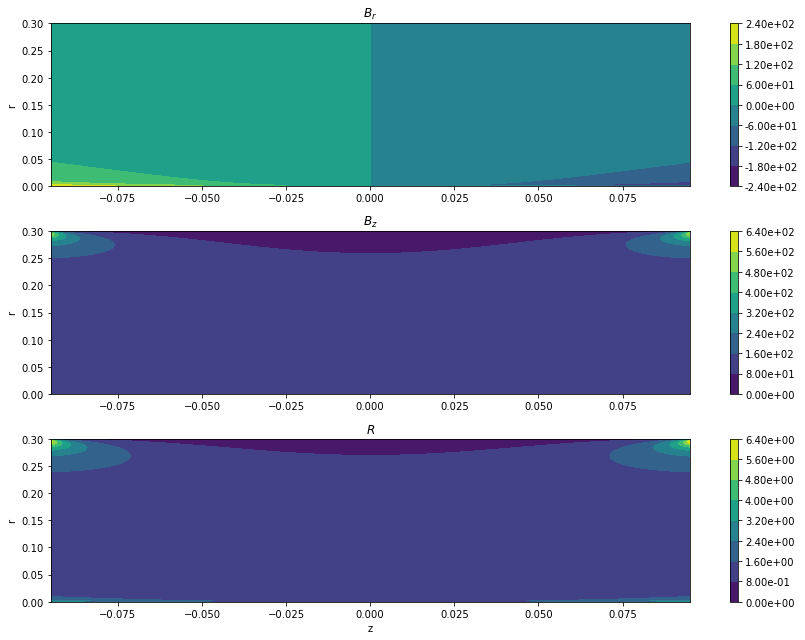
\includegraphics[scale=0.35]
    {L=01.png}}
  \caption{\label{fig:R0.1} Mirror Ratio, a=0.3m, L=0.1m}
\end{figure}
\begin{figure}[h!]
  \center{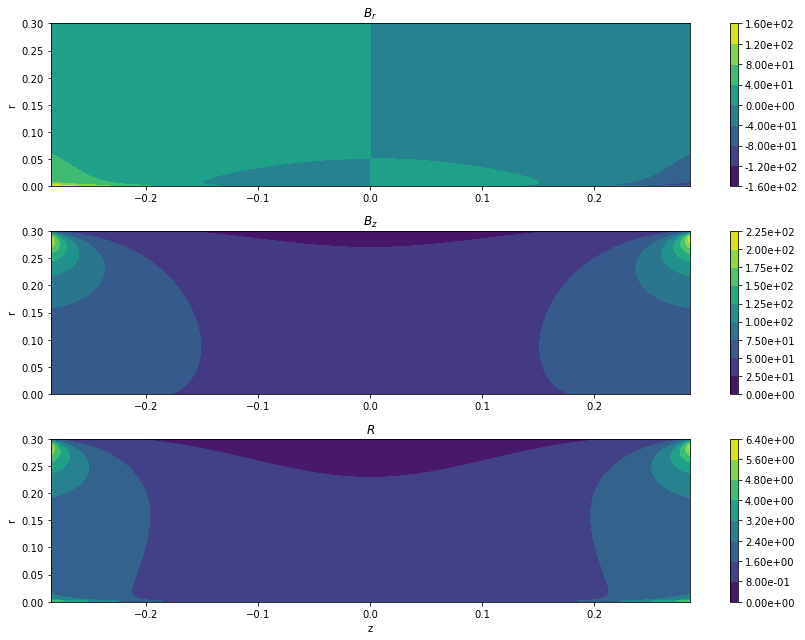
\includegraphics[scale=0.35]
    {L=03.png}}
  \caption{\label{fig:R0.3} Mirror Ratio, a=0.3m, L=0.3m}
\end{figure}
\begin{figure}[h!]
  \center{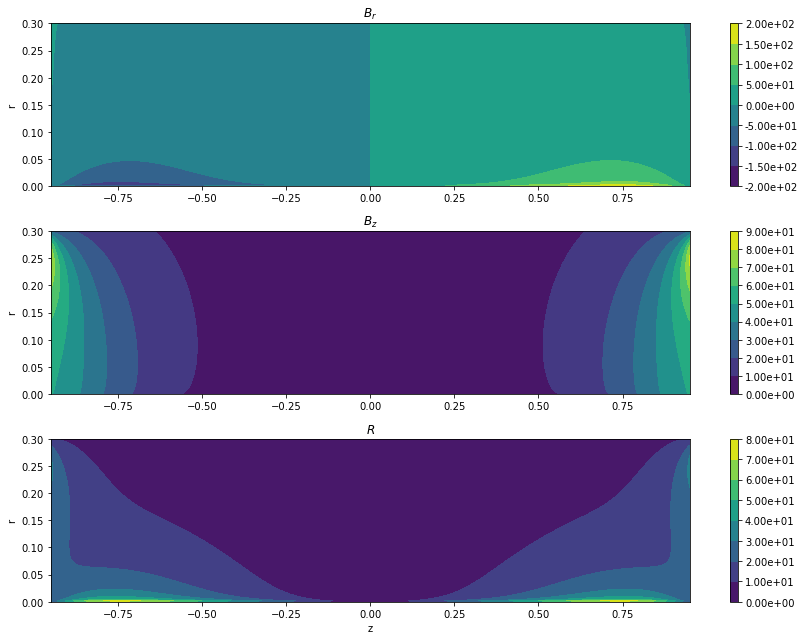
\includegraphics[scale=0.35]
    {L=1.png}}
  \caption{\label{fig:R1} Mirror Ratio, a=0.3m, L=1m}
\end{figure}

These figures were produced using the section of the code which was written by Tal Rubin. As can be seen, the mirror ratio is pretty uniform throughout the middle areas of the mirror, and only changes a lot at the extreme areas, such as at the edge of the coil, or nearing $z=L$. In general, we want the largest possible $R$, and so for most cases, we would choose $L=0.3$. 

The coil fields are very difficult to work with, with pen and paper, so it is common to make approximations. An extremely useful one, takes advantage of the assumption of  a symmetric mirror machine. In this case, there is a minimum at the center, and at that point the first derivative is zero, so the Taylor expansion is simply quadratic:
$$B_z=B_0+B''(0)z^2$$
We can approximate the second derivative as $B_0/L^2$, and so taking into account the requirement for a zero divergence:
\begin{equation}\label{taylorsymB}
\vec{B}=B_0\left(1+\frac{z^2}{L^2}\right)\hat{z}-B_0\frac{rz}{L^2}\hat{r}
\end{equation}
Through a similar procedure, we can also find an approximate field for an asymmetric mirror machine
\begin{equation}\label{taylorasymB}
\vec{B}=B_0\left(1+\frac{z}{L}+\frac{z^2}{L^2}\right)\hat{z}-B_0\left(\frac{r}{2L}+\frac{rz}{L^2}\right)\hat{r}
\end{equation} 
These fields provide quite good approximations to real-world behavior, and they have the nice property of being workable by hand.
\subsection{Relativistic Effects}
In this code's current iteration, it cannot deal with relativistic particles. Therefore, we need to know when a particle becomes relativistic, for the most part I will be using this \href{http://hyperphysics.phy-astr.gsu.edu/hbase/Relativ/rellim.html}{website} as the reference for this section. In general, a good rule of thumb for the limit of non-relativistic theory, is when the error between classical, and relativistic calculations reaches $1\%$. Relativistic kinetic energy is $(1-\gamma)m_0c^2$ where 
\begin{equation}\label{gamma}
\gamma=\frac{1}{\sqrt{1-\frac{v^2}{c^2}}}
\end{equation}
So, this means that the range of energy that is allowed is governed by
\begin{equation}\label{energyrange}
\frac{(1-\gamma)m_0c^2-\frac{1}{2}m_0v^2}{(1-\gamma)m_0c^2}\leq 0.01
\end{equation} 
Which can be solved numerically to find that the allowed $\gamma$ is about $\gamma=1.00673$.
\end{document}